% --------------------------------------------------------------
% This is all preamble stuff that you don't have to worry about.
% Head down to where it says "Start here"
% --------------------------------------------------------------

\documentclass[12pt]{article}

\usepackage[margin=1in]{geometry} 
\usepackage{amsmath,amsthm,amssymb}
\usepackage{multicol} 
\usepackage{tikz}
\setlength{\columnsep}{1cm} % Adjust space between columns
\setlength{\parindent}{0pt} 
\usepackage{array}
\usepackage{geometry}
\geometry{letterpaper} 
\everymath{\displaystyle}
\newcommand{\N}{\mathbb{N}}
\newcommand{\Z}{\mathbb{Z}}

\newenvironment{theorem}[2][Theorem]{\begin{trivlist}
\item[\hskip \labelsep {\bfseries #1}\hskip \labelsep {\bfseries #2.}]}{\end{trivlist}}
\newenvironment{lemma}[2][Lemma]{\begin{trivlist}
\item[\hskip \labelsep {\bfseries #1}\hskip \labelsep {\bfseries #2.}]}{\end{trivlist}}
\newenvironment{exercise}[2][Exercise]{\begin{trivlist}
\item[\hskip \labelsep {\bfseries #1}\hskip \labelsep {\bfseries #2.}]}{\end{trivlist}}
\newenvironment{problem}[2][Problem]{\begin{trivlist}
\item[\hskip \labelsep {\bfseries #1}\hskip \labelsep {\bfseries #2.}]}{\end{trivlist}}
\newenvironment{question}[2][Question]{\begin{trivlist}
\item[\hskip \labelsep {\bfseries #1}\hskip \labelsep {\bfseries #2.}]}{\end{trivlist}}
\newenvironment{corollary}[2][Corollary]{\begin{trivlist}
\item[\hskip \labelsep {\bfseries #1}\hskip \labelsep {\bfseries #2.}]}{\end{trivlist}}

\newenvironment{solution}{\begin{proof}[Solution]}{\end{proof}}

\begin{document}

% --------------------------------------------------------------
%                         Start here
% --------------------------------------------------------------

\title{MATH 116-04 \\ SI Exam Session}
\author{Problem-Solving Strategies}

\maketitle

\subsubsection*{I. Problem-solving strategies}
\vspace{5mm}
In bullet points, detail your problem-solving strategy:
\vspace{40mm}

Describe what you do when you don't even know what to do in a question.
\vspace{40mm}

Imagine what would be the ideal problem solving strategy, write down the strategy in bullets. How does it differ from both strategies described above?

\pagebreak
Here I bulleted some of Terence Tao's advice on solving mathematical problems:
\begin{itemize}
    \item Understand the \textbf{Problem}
    \item Understand the \textbf{Data}
    \item Understand the \textbf{Objective}
    \item Select good \textbf{Notation}
    \item \textbf{Write} everything down
    \item \textbf{Modify} the problem slightly
    \item \textbf{Simplify}, \textbf{exploit} data, and reach tactical \textbf{goals}.
\end{itemize}
\vspace{5mm}
For each of the points, give one example you've encountered before.
Example:



\pagebreak

\pagebreak
\subsubsection*{II. Example of problem}
\begin{center}
   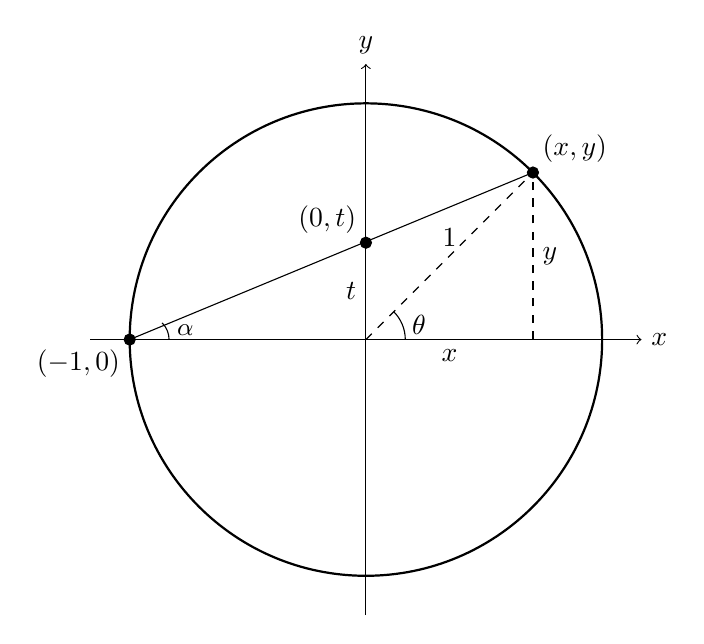
\begin{tikzpicture}
    % Draw axes
    \draw[->] (-3.5, 0) -- (3.5, 0) node[right] {$x$};
    \draw[->] (0, -3.5) -- (0, 3.5) node[above] {$y$};

    % Draw a larger unit circle (radius = 3)
    \draw[thick] (0, 0) circle (3);

    % Define angle theta
    \def\delta{45} % Angle in degrees
    \def\radius{3} % Radius of the circle

    % Calculate (x, y) point on the circle
    \pgfmathsetmacro{\x}{\radius * cos(\delta)}
    \pgfmathsetmacro{\y}{\radius * sin(\delta)}

    % Draw point (x, y) and label it
    \filldraw (\x, \y) circle (2pt) node[above right] {$(x, y)$};

    % Draw line from (x, y) to (0, t)
    \def\t{0} % Define t
    \draw (\x, \y) -- (-3, \t);

    % Draw point (-1, 0)
    \filldraw (-3, 0) circle (2pt) node[below left] {$(-1, 0)$};
    \filldraw (0, 1.23) circle (2pt) node[above left]{$(0, t)$};
    \draw (0, 0) -- (0, 1.23) node[midway, left]{$t$};
    \draw[dashed] (0, 0) -- ({3 * cos(\delta)}, {3 * sin(\delta)}) node[midway, above]{$1$};
    \draw[dashed] ({3 * cos(\delta)}, 0) -- ({3 * cos(\delta)}, {3 * sin(\delta)}) node[midway, right] {$y$};
    \draw[dashed] (0, 0) -- ({3 * cos(\delta)}, 0) node[midway, below] {$x$};
    \draw (0.5, 0) arc (0:45:0.5) node[midway, right] {$\theta$};
    \draw (-2.5, 0) arc (0:45:0.3) node[midway, right] {\small $\alpha$};
\end{tikzpicture}
\end{center}

\begin{itemize}
    \item[\quad \textbf{a.}] Express $\alpha$ in terms of $\theta$. What geometric property justifies this relationship?
    \item[\quad \textbf{b.}] What is the slope of the line $(-1, 0)$ to $(x, y)$ in terms of $t$? And in terms of $x, y$?
    \item[\quad \textbf{c.}] Express $\sin (\theta)$, $\cos{(\theta)}$ and $\tan(\alpha)$ in terms of $t$ using $x^2+y^2=1$ and the slope of part (b).
    \item[\quad \textbf{d.}] Using implicit differentiation, find $d\theta$ in terms of $t$.
    \item[\quad \textbf{e.}] Use the results from parts (c) and (d) to solve the following integral: \[\displaystyle \int \frac{1}{\sin^2{(\theta)}+\cos{(\theta)}+2} \, d\theta\]
\end{itemize}


\subsection*{Reflections}
Go back to the questions and write down your method of solving the exercises in bullet points.
Reflect on how you could improve on your problem solving technique. 

% --------------------------------------------------------------
%     You don't have to mess with anything below this line.
% --------------------------------------------------------------

\end{document}
